%!TEX root = ../thesis.tex
%*******************************************************************************
%****************************** Second Chapter *********************************
%*******************************************************************************

\chapter{Digital pathology and the quantification of immune infiltrate}

\ifpdf
    \graphicspath{{Chapter2/Figs/Raster/}{Chapter2/Figs/PDF/}{Chapter2/Figs/}}
\else
    \graphicspath{{Chapter2/Figs/Vector/}{Chapter2/Figs/}}
\fi

\section[Introduction]{Introduction}
Immune infiltration is frequently manually assessed in pathology departments. Digital pathology is not yet routine in the clinic but increasingly part of modern research as more digital imaging and quantification methods become available. 
Continuous data offers a large number of possibilities for analysis and across the literature there are many approaches. The majority of papers have focused on quantifying epithelial infiltrate alone. Regardless, tissue specific infiltrate requires segmenting the epithelial and stromal compartments and the identification of cells by thresholding for nuclei based on a nuclear stain. The stromal and epithelial immune infiltrate in a tissue section can then be quantified.  In this chapter I worked to complete simple analyses on a dataset from the SEARCH cohort that contained the density of CD$8^+$, CD45RO$^+$ and CD68$^+$ immune cells in epithelium and stroma for each patient and aimed to develop a robust statistical workflow for the analysis of quantitative digital pathology data. I could then expand upon this basic analysis myself and ask questions about model building, the relative importance of stromal and epithelial infiltration, the relationships between them. I aimed to fully investigate, compare and interpret quantities of infiltration in different tissue regions in order to build up a better idea of the compartmental nature of the immune response.

\section{Collaborator Roles}
Anne Montfort (AM) - Sample Sectioning, Staining, Image segmentation\\
JMcD - Pathologist, Image segmentation\\
Anna Piskorz - Sequencing\\
Sarwah Al-Khalidi (SAK) - Resequencing of some samples\\

\subsection{History of the project}
This particular part of the work began from collaboration with AM who approached me with raw files from Definiens image analysis software of CD8$^+$, CD68$^+$ and CD45RO$^+$ stained slides, requiring data cleaning and manipulation and a basic analysis of the relationship between cell count density and survival. 

In this part of the PhD, I utilised this data set to build upon the foundational analysis that I carried out. Firstly investigating the TMAs for bias, extracting and examining the cores that were outlying in size or infiltration. I investigated the distribution of the infiltration densities and normalised them in order to use the correct statistical tests. Along with extracting and modelling the link between immune cell density and survival, I investigated more complex model building. I analysed varying functional forms of infiltrate density, combined multiple infiltrates with principal component analysis for the first time to investigate the underlying patterns of biology and did further analyses including quantifying and assessing the immune exclusion in samples. I also applied some similar analyses to the other subtypes of Ovarian Cancer in the cohort.

\begin{figure}
    \centering
    \includegraphics{Chapter2/Figs/Raster/Thesis_visual_abstract.PNG}
    \caption[Visual Abstract]{Visual abstract}
    \label{fig:visual_abstract}
\end{figure}

\section{SEARCH Cohort}

Samples from 570 patients from the prospective SEARCH ovarian cancer population-based study had been used to construct tissue microarrays. Ethical approval was granted by the Eastern Multicenter Research Ethics Committee. Among the samples from 570 patients with primary epithelial ovarian tumours, 332 were high grade serous ovarian cancer patients. All cases underwent detailed histopathological review by a gynaecological pathologist (JM). Patients were staged as having localized, regional or distant disease (L/R/D).

\section[Methods]{Methodology}
\subsection{SEARCH Data Set}
As mentioned, the immunohistochemical staining and initial utilization of Definiens software was carried out by AM. The methodology used to acquire the data set used in this section is outlined below and referred to in detail in the Methods chapter. 

\subsubsection{Immunohistochemistry}
Immunohistochemistry on the SEARCH samples was carried out upon the tissue sections by Anne Montfort (AM) according to the protocol in section \ref{sec:am_method}. Previously published PTEN immunostaining data was used where high PTEN expression was considered to be positive staining and low expression to be weak, heterogeneous or negative staining respectively\cite{RN17}.

\subsubsection{\texit{TP53} mutation data}

Sequencing and mutation analysis was carried out prior to this PhD by Anna Piskorz (AP). The coding regions of \textit{TP53} were sequenced by tagged-amplicon next generation sequencing (TamSeq) as previously described\cite{RN18} and confirmed by immunohistochemical analysis using a 4-tier core system\cite{RN19}. Sequencing of germline mutations in the  \texit{BRCA1} and \texit{BRCA2} genes was performed as previously described\cite{RN20}. Some samples were resequenced using TamSeq by SAK following my initial exploratory analysis and datacleaning steps. The results of resequencing were integrated into the final analysis.

\subsubsection{Immune cell quantification}
 The number of CD8$^+$ and CD45RO$^+$ cells in epithelial and stroma areas, the area of epithelial and stromal areas covered by CD68 staining and the total area of epithelium and stroma in each core, had been digitally determined using the Tissue Studio software (Definiens™).

Figure \ref{fig:segmentation} shows examples of this cell segmentation and tissue classification.

\begin{figure}[htbp!] 
\centering    
\includegraphics[width=0.8\textwidth]{Chapter2/Figs/Raster/Segmentation.png}
\caption[Segmentation in Definiens]{Examples of the segmentation of tissues and identification of cells in the Definiens software.}
\label{fig:segmentation}
\end{figure}

\subsection{Statistical analyses}
 The clinical variables of age at diagnosis, menopause status and stage were available for the cohort and I included them in the analysis. I used univariable Cox regressions to identify best-fitting variables for the final multivariable Cox regression model. The refined model was compared with a combined multivariable Cox regression model including all immune infiltrates. Hazard ratios (HR) refer to a single unit increase in continuous variables. The proportional hazards assumption was tested and satisfied in all cases using Schoenfeld residuals. The Kaplan–Meier analysis (with log-rank test) was applied to illustrate survival differences graphically. Two-sided P-values <0.05 were used to indicate statistical significance. 

Principal component analysis (PCA) using the R package \textbf{prcomp} was used to extract the independent components of variance between patients. The package \textbf{prcomp} uses singular value decomposition and the variables were scaled to have unit variance before creating composite linear independent variables. These were then passed forward to the survival modelling. The Akaike Information Criterion (AIC), equation \ref{eq:AIC} was used to compare the performance of survival models.

Bonferroni p-value corrections were carried out for all multiple testing. P < 0.05 was considered significant for all analyses. 


\section{Results}
 
 The SEARCH cohort included patients with HGSOC, Clear Cell, Endometrioid, Mucinous and Low Grade Serous Ovarian Cancer. These subtypes of Ovarian Cancer have vastly different cells of origin, different patterns of infiltration and different genomic drivers. As I was primarily interested in understanding the differences within populations rather than across subtypes, I extracted the HGSOC subpopulation for the initial analysis.

\subsection{Patient characteristics}
Figure {\ref{fig:remark_search}} shows the REMARK diagram for this study and Table \ref{table:clinical_SEARCH} shows the clinical characteristics of the 332 HGSOC patients from the study cohort. Immunohistochemical analyses on tissue microarrays (TMAs) were performed to detect CD8$^+$, CD45RO$^+$ and CD68$^+$ cells in tissue cores from primary ovarian specimens.  152 HGSOC cases were available for analysis after quality assurance, data cleaning and the reduction of the data set to only cases with complete results for CD8, CD45RO and CD68 staining in both epithelium and stroma as well as survival data. 
Tagged amplicon sequencing data was available for 248 cases and \textit{TP53} mutation was detected in 231 samples (93\%) (Table \ref{tab:clinical_SEARCH}). Previously published data for germline  \texit{BRCA1} and \texit{BRCA2} mutation and PTEN expression were available for 297 and 155 cases respectively\cite{17,20}.

\begin{figure}
    \centering
    \includegraphics[width=0.8\textwidth]{Chapter2/Figs/Raster/montfort-REMARK.png}
    \caption{REMARK diagram for the SEARCH cohort.}
    \label{fig:remark_search}
\end{figure}
\begin{table}[]
    \centering
    \begin{tabular}{lll}
    \hline
 N	&	& 332 \\
Median Age (IQR) & & 58.0 (51.0-64.0) \\
\hline
Stage &	localized &	64 (19.3\%)\\
 &	regional &	42 (12.7\%)\\
 &	distant	& 202 (60.8\%)\\
 &	unstaged &	24 (7.2\%)\\
 \hline
TP53 mutation &	gof &	137 (55.2\%) \\
 &	lof &	94 (37.9\%)\\
&	wild type &	17 (6.9\%)\\
 &	Not assessed &	84 \\
 \hline
PTEN IF	& 	High &	28 (18.1\%)\\
& 	Low	 & 127 (81.9\%)\\
&	Not available &	177 \\
\hline
BRCA status		& 	wild type &	256 (86.2\%)\\
 &	\textit{BRCA1} &	18 (6.1\%)\\
 &	\texit{BRCA2} &	23 (7.7\%)\\
 &	Not available &	35\\
\hline
    \end{tabular}
    \caption{Patient characteristics for the HGSOC subset of the SEARCH cohort.}
    \label{tab:clinical_SEARCH}
\end{table}

 \subsection{Data cleaning, quality assurance and spatial bias}

Analysing a large number of digitally imaged and segmented TMA cores gave me the ability to carry out quality checking for bias across TMAs and to evaluate the variation in properties of the tissue core such as tissue area, something typically not measured by pathologists when assessing cores manually.

I examined the distribution of tissue area and ensured that the varying tissue area across TMAs was random \ref{fig:area_dist}. I did this visually using heatmaps (Figure \ref{fig:heatmap_area}) and statistically using Shapiro-Wilk tests ($p > 0.05 $). 

\begin{figure}
    \centering
    \includegraphics[width=0.8\textwidth]{Chapter2/Figs/Raster/area_heatmap.png}
    \caption{Heatmap of total core area across TMA.}
    \label{fig:heatmap_area}
\end{figure}

\begin{figure}
    \centering
    \includegraphics[width=0.4\textwidth]{Chapter2/Figs/Raster/Area_distribution_hist.png}
    \caption{The distribution of total tissue area for each core in the SEARCH cohort.}
    \label{fig:area_dist}
\end{figure}
 
As mentioned, CD8$^+$ and CD45RO$^+$ counts were initially calculated as number of cells in stroma and epithelium and CD68$^+$ scoring was given as area covered. I processed this raw data, converting cell counts into cells per unit area and CD68$^+$ coverage into percentage area. This normalization to area allows for comparison between patients whose tissue is made up of varying quantities of stroma and epithelium. I also confirmed using  residuals that transforming the count densities to base 10 would normalize them.


I also extracted outlying examples of cores to ensure the despite the tissue area sampled varying, that the measures of infiltrate density were not significantly different from the population as a whole. Figure \ref{fig:heatmap} shows a heatmap comparing infiltration density across the CD8$^+$ , CD68$^+$ and CD45RO$^+$ TMAs. No spatial relationship was observed over a single TMA between the location of a core and the density of immune cells or the tissue area. 



\begin{figure}
    \centering
    \includegraphics{Chapter2/Figs/Raster/Thesis-heatmap.png}
    \caption{Density of each infiltrate for each position in the SEARCH TMA.}
    \label{fig:outlying_core}
\end{figure}


\subsection{Stroma and tumour composition of cores}
Digital pathology and tissue segmentation provides a unique opportunity to evaluate stromal and epithelial areas and the makeup of sampled tissue cores. An example of the segmentation used to generate this data set is shown in Figure \ref{fig:segmentation}.  Pathologists sample tissue from sections of FFPE blocks for the construction of TMAs. Other than aiming to sample regions with high percentages of epithelium, this sampling is otherwise uncontrolled. I wanted to investigate the variation in epithelial and stromal tissue that was sampled in the SEARCH TMAs. The distribution of epithelial and stromal areas are shown in Figure \ref{fig:distribution_infiltrate}. \\

\begin{figure}
    \centering
    \includegraphics{Chapter2/Figs/Raster/Montfort-2018_epi_stroma_dist.png}
    \caption{The distribution of epithelial and stromal areas.}
    \label{fig:distribution_infiltrate}
\end{figure}

I found that of 964 images representing 332 HGSOC patients, 69 patients (20.8\%) had images which contained malignant epithelium but no stroma; 250 patients (75.3\%) had images which contained epithelium and >1\% adjacent stroma and 13 patients (3.9\%) had images containing no tumour epithelium (Fig \ref{fig:distribution_infiltrate}). The median proportion of epithelium and stroma was 85.1\% (IQR 51–100\%) and 14.9\% (IQR 0–49\%) respectively.

\subsection{Mutant allele fraction and epithelial content}

In order to perform a quality check on cores I utilised the side data set from this cohort of the mutant allele fraction for all samples. The distribution of mutant allele fraction is plotted as a histogram in  Figure \ref{fig:maf_dist}. I used this to ensure that the sequencing of all samples classified as HGSOC was of high enough quality. Samples with mutant allele fraction of zero were resequenced and if no mutation was found were excluded from HGSOC analysis.
\begin{figure}
    \centering
    \includegraphics[width=0.4\textwidth]{Chapter2/Figs/Raster/MAF_distribution.png}
    \caption{Histogram of counts of samples against mutant allele fraction.}
    \label{fig:maf_dist}
\end{figure}

 As p53 mutations are found ubiquitously in HGSOC we would expect that the proportion of epithelial cells in a sample is correlated with \textit{tp53} mutant allele fraction.  I found them to be positively correlated ($R= 0.24$, $p=0.0027$). The sequencing and imaging are not carried out on exactly the same tumour region and so I would not expect a perfect correlation due to natural noise from sampling. The correlation between technical replicates for allele frequency and sequencing depth is shown in Appendix \ref{fig:p53_allele}. 
\begin{figure}
    \centering
    \includegraphics{Chapter2/Figs/Raster/maf_epithelial.png}
    \caption{\textit{p53} mutant allele fraction against epithelial area of a core.}
    \label{fig:p53_allele}
\end{figure}




\subsection{Immune cell densities}

An example of the assessment of CD8$^+$ T cell, CD45RO$^+$ memory lymphocyte and CD68$^+$ macrophage densities and the allocation of the stromal and epithelial regions is shown in Fig. \ref{fig:segmentation}.

As demonstrated, cores frequently sample varying areas of epithelium and stroma and therefore sample different proportions of epithelial and stromal infiltrate. In order to understand the impact of this sampling I felt that it was important to know how the density of infiltration varies between epithelial and stromal compartments. The distribution of densities of immune populations within tumour epithelium and stromal areas were compared (Fig. \ref{fig:distribution_infiltrate}). I found that the density of CD8$^+$ and CD45RO$^+$ cells were significantly higher in stroma than tumour epithelium (p = 0.005 and p = 0.004 respectively; Welch’s t-test) but not significantly different for CD68$^+$ cells. 

\begin{figure}
    \centering
    \includegraphics[width=\textwidth]{Chapter2/Figs/Raster/Montfort-2018_immune_Composition.png}
    \caption[Distribution of immune densities.]{ (A), (B) and (C) show the distribution of CD8$^+$, CD45RO$^+$ and CD68$^+$ immune cell densities in epithelium and stroma. CD8$^+$ and CD45RO$^+$ densities were defined as counts per mm2 and CD68$^+$ as the percentage of tissue stained for this marker. (Notches on box plots extend 1.58 ✕ IQR / sqrt(n) and approximate the 95\% confidence interval for the median. Box plot whiskers extend to 1.5 ✕ IQR.) 
}
    \label{fig:distribution_infiltrate}
\end{figure}

The predominant population of immune cells studied in the literature is epithelial CD8$^+$ infiltrate which has been demonstrated to have a log-linear relationship with survival. In order to evaluate the true nature of this infiltration in the microenvironmental context I investigated whether this infiltrate was independent of others. If this infiltrate is not independent, the survival impact may be an indirect readout of the presence of other infiltrates. The correlation between infiltrates is also important to understand whether there exist spatial dynamics of infiltration and the relationship and movement between adjacent tissue compartments. The quantitative measure of immune density in our samples allowed me to investigate the pearson correlation between quantities of immune infiltrate. The quantity of the three immune populations in this cohort showed moderate to strong correlation between infiltrate in epithelium and stroma and between the three infiltrates (Figure \ref{fig:ch2_correlation} and Table \ref{tab:cor_pvals}). 

\begin{figure}
    \centering
    \includegraphics[width=0.8\textwidth]{Chapter2/Figs/Raster/correlation_inf.png}
    \caption[Correlation between infiltrates]{Scatterplots and distributions of CD68$^+$, CD45RO$^+$ and CD8$^+$ infiltrate in Stroma and Epithelium. The quantities of all infiltrates were correlated between matched samples across both tissue region classes.}
    \label{fig:ch2_correlation}
\end{figure}

Given that we see varying epithelial cell percentages and increased infiltrate in the stroma as compared with the tumour I was interested in whether the density of immune infiltrate reaching the epithelium was related to the epithelial percentage of the core. In  other words, does increasing the quantity of tumour in a sample increase the infiltration, perhaps due to the presence of more tumour antigens and therby more immune cell recruitment or decrease it due to reduced stromal access and infiltration. I examined the relationship between the fraction of tumour in a core and the density of immune infiltration in the epithelium using Pearson correlation test. Intra-epithelial CD8$^+$ and CD45RO$^+$ densities were  weakly positively correlated with the purity/tumour fraction of the sample ($R^2 = 0.17$, $p = 0.003$ and $R^2 = 0.16$, $p=0.006$) whereas CD68$^+$ epithelial density was not.



\subsection{Immune exclusion}

When considering patterns in immune infiltration, beyond the binary of present and absent, the terms immune-inflamed, immune-desert and immune-excluded have been used to describe varying T-cell infiltration based on histological and transcriptional analyses \cite{}. Immune-inflamed and immune-desert patterns reflect high positive or negative correlations between all infiltrates but T-cell exclusion describes tumours where CD8$^+$ cells are significantly absent from tumour epithelium whilst still being present in the surrounding stroma\cite{,27}. 

On average there is more infiltration in the stroma than epithelial compartments as shown in Figure \ref{fig:distribution_infiltrate} but the plot in Figure \ref{fig:ratio} shows that the ratio of epithelial:stromal infiltration is log-normal. As the counts are log-transformed, the ratio of infiltration density is equal to the difference between the logs of the epithelial and stromal infiltration. I defined this ratio as the extent of epithelial exclusion. The standard deviation of the ratio of CD8+ and CD45RO+ epithelial:stromal infiltration were both 0.68.

19 (10.1\%) cases had 10x as much stromal infiltration as epithelial CD8$^+$ cases and 39 (20.5\%) cases had 10x as much stromal CD45RO$^+$. 3 cases had 10x as much CD68$^+$ infiltrate as epithelial infiltrate.  All ratios were normally distributed and the CD8$^+$ and CD45RO$^+$ exclusion was weakly correlated ($R=0.2, p=0.009$).   %Expand on why I used 10 fold cut off etc, examine cutoffs etc and differences. INCLUDE PLOT.

\begin{figure}
    \centering
    \includegraphics[width=0.5\textwidth]{Chapter2/Figs/Raster/Figurenew_ratio_scatter.png}
    \caption{Immune exclusion ratio of CD8 and CD45RO T-cells. Ratios are log-transformed like the counts. Histograms of exclusion are shown on the graph, both distributions are log-normal.}
    \label{fig:ratio}
\end{figure}



\subsection{Functional form of infiltrates in building a survival model}
When modelling survival using Cox regression, one must assess that the assumptions of the Cox model are met and decide upon the functional form of the predictor\ref{eq:cox}. I utilized Martingale residuals (Figure \ref{fig:martingale} to confirm that the base 10 transformation previously applied successfully addressed the non-linearity of the data. In order to find the best functional form for each predictor I modelled the univariate relationship between the predictor and survival using Cox regression and plotting the residuals of the model fit against the expected form. The relationship between each of the immune variables and survival was found to be approximately log-linear. 

\begin{figure}
    \centering
    \includegraphics{Chapter2/Figs/Raster/martingale_plots.png}
    \caption{Martingale residuals of each infiltrate assesses the linearity of the variables. The log10 transformation is seen to improve linearity in all cases.}
    \label{fig:martingale}
\end{figure}

The only clinical variables accompanying the cohort were age at diagnosis, stage and menopause status. Age at diagnosis is the only continuous variable of these and the relationship between age and survival was found to be approximately linear (Figure \ref{fig:modelfit}, Table \ref{tab:model_fit}). 

\begin{table}[]
    \centering
    \begin{tabular}{cccc} \hline
        	&	Linear 	&	Cubic splines	&	Log(base 10)	\\
	&	p-value	&	p-value	&	p-value	\\ \hline
Age at diagnosis	&	0.18	&	0.36	&	0.24	\\
CD8$^+$ epithelium	&	0.43	&	0.36	&	0.25	\\
CD8$^+$ stroma	&	0.4	&	0.17	&	0.64	\\
CD68$^+$ epithelium	&	0.44	&	0.57	&	0.63	\\
CD68$^+$ stroma	&	0.09	&	0.06	&	0.009	\\
CD45RO$^+$ epithelium	&	0.3	&	0.09	&	0.07	\\
CD45RO$^+$ stroma	&	0.07	&	0.016	&	0.002	\\
\hline

    \end{tabular}
    \caption[P-values for the association of each functional form of the variable with survival]{P-values for the association of each functional form of the variable with survival using univariable Cox regression analyses. Lowest p-values demonstrate most likely functional form and show that each relationship is approximately log linear}
    \label{tab:model_fit}
\end{table}

\begin{figure}
    \centering
    \includegraphics[width=\textwidth]{Chapter2/Figs/Raster/Artboard 39.png}
    \caption[Residuals of model fit]{Residuals of model fit plotted against predicted value for age at diagnosis, the relationship was found to be approximately linear.}
    \label{fig:model_age}
\end{figure}



\subsection[Prognostic value of individual infiltrates]{Stromal CD68$^+$ and CD45RO$^+$ infiltrate are the strongest individual prognostic markers}

Initially I investigated whether survival models of the individual infiltrates in stroma and tumour accurately fit the data. Univariable analysis showed improved survival with increasing stromal density of CD45RO$^+$ (HR 0.76 95\% CI 0.65–0.90, p=0.001) and CD68$^+$(HR 0.53 95\% CI 0.34–0.81, p=0.003) (Table \ref{tab:coxsurv}). Modelling each immune variable with stage showed improved predictive value for epithelial CD8$^+$ density (HR=0.83, p-value=0.027) as well as stromal CD68$^+$ and CD45RO$^+$ density and epithelial CD45RO$^+$ density (Table  \ref{tab:coxsurv}). Kaplan-Meier curves require an arbitary cutpoint for continuous data that impacts reported significance, as such I used these for illustrative purposes only. Figure \ref{fig:kmcd68845}) shows illustrative Kaplan-Meier survival curves for high and low stromal and epithelial CD68$^+$, CD45RO$^+$ and CD8$^+$ densities.\\



\subsection{Averaging immune infiltrate over a core}

In clinical reporting, quantifying immune populations in exclusively tumour epithelium is technically challenging and time consuming. I was therefore interested in testing the value of using the average density of each marker averaged across both tumour and stromal regions from each core (Table \ref{tab:coxsurv}).  Averaging the tissue density of CD8$^+$ increased the strength of the associated hazard ratio and significance of the model (HR=0.79, p-value=0.010) indicating increased prognostic value for CD8$^+$ infiltrate over quantitation of individual epithelial and stromal infiltrates. The significance did not increase for CD45RO$^+$ and CD68$^+$ infiltrates.  Figure \ref{fig:KM_infiltrates} shows illustrative Kaplan-Meier survival curves for high and low CD68$^+$, CD45RO$^+$ and CD8$^+$ densities over combined epithelium and stroma compartments.\\


\begin{landscape}
\begin{table}[]
    \centering
    \begin{tabular}{llllllll}
    
		& & &&		Univariable && \multicolumn{2}{c}{	Multivariable* 
(adjusted for stage)} \\
								
&	Functional Form &	Evaluable cases&	Tissue compartment&	HR &	p-value	& HR &	p-value	\\ \hline
CD8$^+$&	log10 &	301	&Epithelium&	0.89&	0.15&	0.83&	0.027\\	
&	log10&	202&	Stroma&	0.97&	0.74&	0.93&	0.40\\	
&	log10&	315&	Average&	0.79&	0.010&	0.72&	0.0006\\	
CD45RO+&	log10&	290&	Epithelium&	0.86&	0.033&	0.85&	0.022\\	
	&log10&	196&	Stroma&	0.76&	0.001&	0.76&	0.0007\\	
	&log10&	306&	Average&	0.82&	0.006&	0.80&	0.003\\	
CD68+&	linear&	293&	Epithelium&	0.99&	0.67&	0.99&	0.43\\	
&	log10&	226	&Stroma	&0.53&	0.003&	0.44&	0.0003	\\
&	log10&	308	&Average&	0.67&	0.042&	0.62&	0.017\\	
Stage1 & - &	312&	Localised&	1&	0&	1&	0	\\
	& & &		Regional&	1.47&	0.26&	1.15&	0.25\\	
	&	&&	Distant	&3.96&	<<0.001&	5.58&	<<0.001	\\
	&	&&	Unstaged&	3.35&	<0.001&	3.34&	<<0.001	\\ \hline

\end{tabular}
    \caption[Individual immune infiltrates Cox regression]{Cox proportional hazards survival analysis for individual infiltrates.}
    \label{tab:coxsurv}
\end{table}
\end{landscape}

\begin{figure}
    \centering
    \includegraphics{Chapter2/Figs/Raster/KM_allinf.png}
    \caption[KM Survival curves for individual infiltrates]{Kaplan–Meier survival curves using cut point of median density of stromal CD68$^+$ macrophages and CD45RO$^+$ memory T cells using left truncation and right censoring. Median entry to the study for all patients after diagnosis was 26.4 months. Median follow up time from diagnosis to exit or death was 105.1 months.}
    \label{fig:KM_infiltrates}
\end{figure}

\subsection{Epithelial core subset survival analysis}

Alongside assessing cores with both tumour and stroma and consequently assessing the survival impact of immune cells in a stromally infiltrated environment, I wanted to test these associations in purely epithelial cores. I asked whether CD45RO$^+$ and CD8$^+$ epithelial infiltrate were still significant predictors in predominantly epithelial cores. In the separate subset of cores with <1\% stroma, epithelial CD8$^+$ malignant epithelial infiltrate remained an independent prognostic factor but epithelial CD45RO$^+$ density was not significant (n=110,p=0.78)(Table \ref{tab:surv_cd8_epi}).

\begin{table}[]
    \centering
    \begin{tabular}{cccccc}\hline 	&		&	\multicolumn{2}{l}{Univariable}			&	\multicolumn{2}{l}{Multivariable*}			\\
 	&	Cases	&	HR	&	p-value	&	HR	&	p-value	\\ \hline
CD8+	&	111	&	0.84	&	0.27	&	0.7	&	0.047	\\
CD45RO+	&	110	&	0.98	&	0.89	&	0.96	&	0.78	\\
CD68+	&	80	&	1.21	&	0.47	&	1.27	&	0.39	\\
\hline
    \end{tabular}
    \caption[Epithelial core immune infiltrate and survival]{Cox proportional hazard regression for cores with malignant epithelial tissue only. Multivariable analysis includes stage.}
    \label{tab:surv_cd8_epi}
\end{table}


\subsection{Combined model}

Given that individually, all infiltrates were prognostic in at least one compartment, the next step was to model the survival of patients based on all infiltrates together to account for the different effects of differing infiltrates. I carried out multivariable Cox regression analysis including all infiltrates and stage on patients with complete data for all infiltrates (n=152) (Table \ref{tab:cox_combined}).  In this model only stage and CD68$^+$ stromal infiltrate were significant predictors of survival.

I then refined the model by removing the least significant elements (defined as those with p>0.1) (Table \ref{tab:cox_combined}, n=152). Interestingly, I found that the p-values for CD68$^+$ and CD45RO$^+$ stromal infiltrates in the refined model become less significant and the hazard ratios are attenuated in comparison to both the univariable regression and the full model. This is likely due to the inability of Cox regression to distinguish with confidence whether stromal CD45RO$^+$ or CD68$^+$ density is the most significant predictor when there is a strong correlation between all the immune variables.
\begin{table}[]
    \centering
    \begin{tabular}{llcccc} \hline
&&	Multivariable & (all combined) &	Refined model &\\ 
	&&	HR&	p-value&	HR&	p-value\\ \hline
CD8+&	Epithelium&	0.96&	0.81&	-	&-\\
	&Stroma&	1.07	0.63	&-&	-\\
CD45RO+&	Epithelium&	1.12&	0.37	&-&	-\\
	&Stroma	&0.83	&0.09	&0.68&	0.11\\
CD68+&	Epithelium&	1.16&	0.63	&-&	-\\
	&Stroma	&0.53&	0.038&	0.88	&0.17\\
Stage &&&&&\\
&Localised&	1&	0&	1&	0\\
&	Regional&	2.00&	0.16&	2.03&	0.14\\
&	Distant&	4.82&	<<0.001&	4.70&	0.0001\\
&	Unstaged	&8.15&	<<0.001&	8.25&	0.0001\\ \hline

    \end{tabular}
    \caption[Cox regression HR and p-values for combined and reduced survival models.]{Cox proportional hazard regression HR for combined and reduced models. The Refined model is reduced down from all infiltrates to attempt to improve the model. Stage is included in both models.}
    \label{tab:cox_combined}
\end{table}

\subsection{Is the ratio of stromal T-cell infiltrate to intra-epithelial T-cell infiltrate prognostic?}

Immune exclusion and the location of immune infiltrate in either the intra-epithelial or stromal regions is a spatial micro-environmental property that can easily be derived from images. The ratio of tumour to stromal infiltrate may indirectly measure properties of the ECM that allow for infiltration into the tumour core or measure the extent of the interaction of the immune cells with epithelial cells. As shown previously, stromal and intra-epithelial immune cell densities are correlated. I investigated whether the ratio of stromal infiltrate density to intra-epithelial immune infiltrate density was a significant predictor of risk in HGSOC using the Cox proportional hazards model.

% latex table generated in R 3.3.2 by xtable 1.8-2 package
% Thu Oct 19 15:01:03 2017
\begin{table}[ht]
\centering
\begin{tabular}{llllll} \hline
 	&		&	\multicolumn{2}{l}{Univariable}			&	\multicolumn{2}{l}{Multivariable}			\\
 	    &	n	&	HR	&	p-value	    &	HR	&	p-value	\\ \hline
CD8	    &	188	&	0.94	&	0.65	&	0.95	&	0.69	\\
CD45RO	&	180	&	1.13	&	0.36	&	1.28	&	0.20	\\
CD68	&	211	&	1.53	&	0.09	&	1.54	&	0.018	\\

   \hline
\multicolumn{5}{l}{}\\
\end{tabular}
\caption[Cox regression for ratio of Tumour to Stroma infiltrate]{Single predictor Cox proportional hazard tests with ratios of stromal to tumour infiltrate as predictors.} 
\label{tab:s:t}
\end{table}
There is no significant effect on survival of stroma:tumour ratio for the T-cell subsets. The ratio of tumour:stroma macrophages however has an impact upon survival, with a higher epithelial:stromal infiltration ratio having a negative impact upon survival (Table \ref{tab:s:t}, $p=0.018, \mathrm{HR}=1.54$).

\subsection{Principal components and the combined immunospace}
 Part of the problem that I encountered in analysing the effect of multiple immune populations upon survival is that the multiple immune infiltrates are correlated (see Figure \ref{fig:ch2_correlation}) and may have additive or suppressive effects.  In order to assess the multi-dimensional nature of the immune response in more detail I proposed that as the three types of immune infiltrate vary continuously across epithelium and stroma these variables can be regarded as six dimensions of an ‘immunospace’ (three infiltrates, 2 localizations).  Given the strong correlations between infiltrates (Figure \ref{fig:ch2_correlation}), we can safely say these immune variables are not independent. I used principal component analysis (PCA) to determine the independent patterns across these dimensions, using the 152 patients for whom complete data were available.
 
 PCA transformed the six correlated infiltrate variables into six independent axes with the first component containing the largest proportion of variance (60\%) in the data set\ref{tab:PC}. Patients are plotted by their PC1 and PC2 values in Figure \ref{fig:PC_plot}. In principal component 1 (PC1), the weightings of all immune infiltrates are positive and similar in magnitude (Table \ref{tab:PC}). This indicates that as one infiltrate increases so do all the others and represents the degree of coordinated immune response. The remaining principal components characterize additional patterns across immune infiltrates independent of PC1. The additive contribution of PC2 characterises negative correlation between CD8$^+$ infiltrates and CD68$^+$ macrophages and CD45RO$^+$ memory cells. PC3 characterizes additional variation where epithelial and stromal infiltrates are negatively correlated, the most positive values of PC3 correspond to high infiltration in tumour epithelium compared to stroma and the most negative values of PC3 correspond to the opposite, the aforementioned immune exclusion. 
 
\begin{table}[]
    \centering
    \begin{tabular}{lllllll}\hline
&PC1& PC2&PC3&PC4&PC5&PC6\\
&(60\%)&(13\%)&(9\%)&(8\%)&(5.5\%)&(4.5\%)\\
\hline
CD8$^+$ tumour density& 0.38&-0.56&0.58&-0.1&0.4&-0.21\\
CD8$^+$ stromal density&0.38&-0.59&-0.47&0.27&-0.21&0.43\\
CD68$^+$ tumour density&0.41&0.47&0.37&0.11&0.09&0.67\\
CD68$^+$ stromal density&0.42&0.3&-0.29&0.56&0.36&-0.45\\
CD45RO$^+$ tumour density&0.45&0.11&0.21&-0.07&-0.78&-0.36\\
CD45RO$^+$ stromal density&0.41&0.15&-0.42&-0.77&0.22&-0.03\\
\hline
    \end{tabular}
    \caption[Composition of the principal components across all infiltrates]{Contributions of normalized infiltrates to all principal components. Figures in brackets indicate proportion of total variance}
    \label{tab:PC}
\end{table}

\begin{figure}
    \centering
    \includegraphics{Chapter2/Figs/Raster/PCA_xy.png}
    \caption{Patients plotted on axes giving their values of Principal Component 1 and 2.}
    \label{fig:PC_plot}
\end{figure}
 
Having calculated the principal components from the data, it is possible to extract the patients who lie at the most extreme ends of these axes of variation. Figure \ref{fig:PC_examples} shows representative images with the largest magnitudes of PC1, PC2 and PC3 to visually illustrate the patterns described above. This figure demonstrates especially clearly the coordinated immune infiltration and the immune exclusion that are described by PC1 and PC3. 

The variance in the remaining principal components (4-6) is smaller and less informative. Variance in PC4 is predominantly from CD45RO$^+$ stromal density, PC5 is from CD45RO$^+$ epithelial density and PC6 is from CD68$^+$ epithelial density. 


In order to evaluate the prognostic impact of these patterns of infiltration, I used Cox proportional hazard regression to assess whether these principal components were predictive of survival. Cox regression survival models were also calculated on all combinations of principal components and stage. Only PC1 was an independent predictor of survival in this cohort and was associated with improved survival (Univariate: HR=$0.89$, $p=0.024$, PC1+Stage: HR: $0.88$, $p=0.019$) (Table \ref{tab:pc_surv}) reflecting the good prognosis of a strong coordinated immune response. The association of this principal component with survival is also illustrated graphically using Kaplan Meier curves in Fig. \ref{fig:km_PC}.

\begin{landscape}
\begin{figure}[width=0.8\textwidth, keepaspectratio]
    \centering
    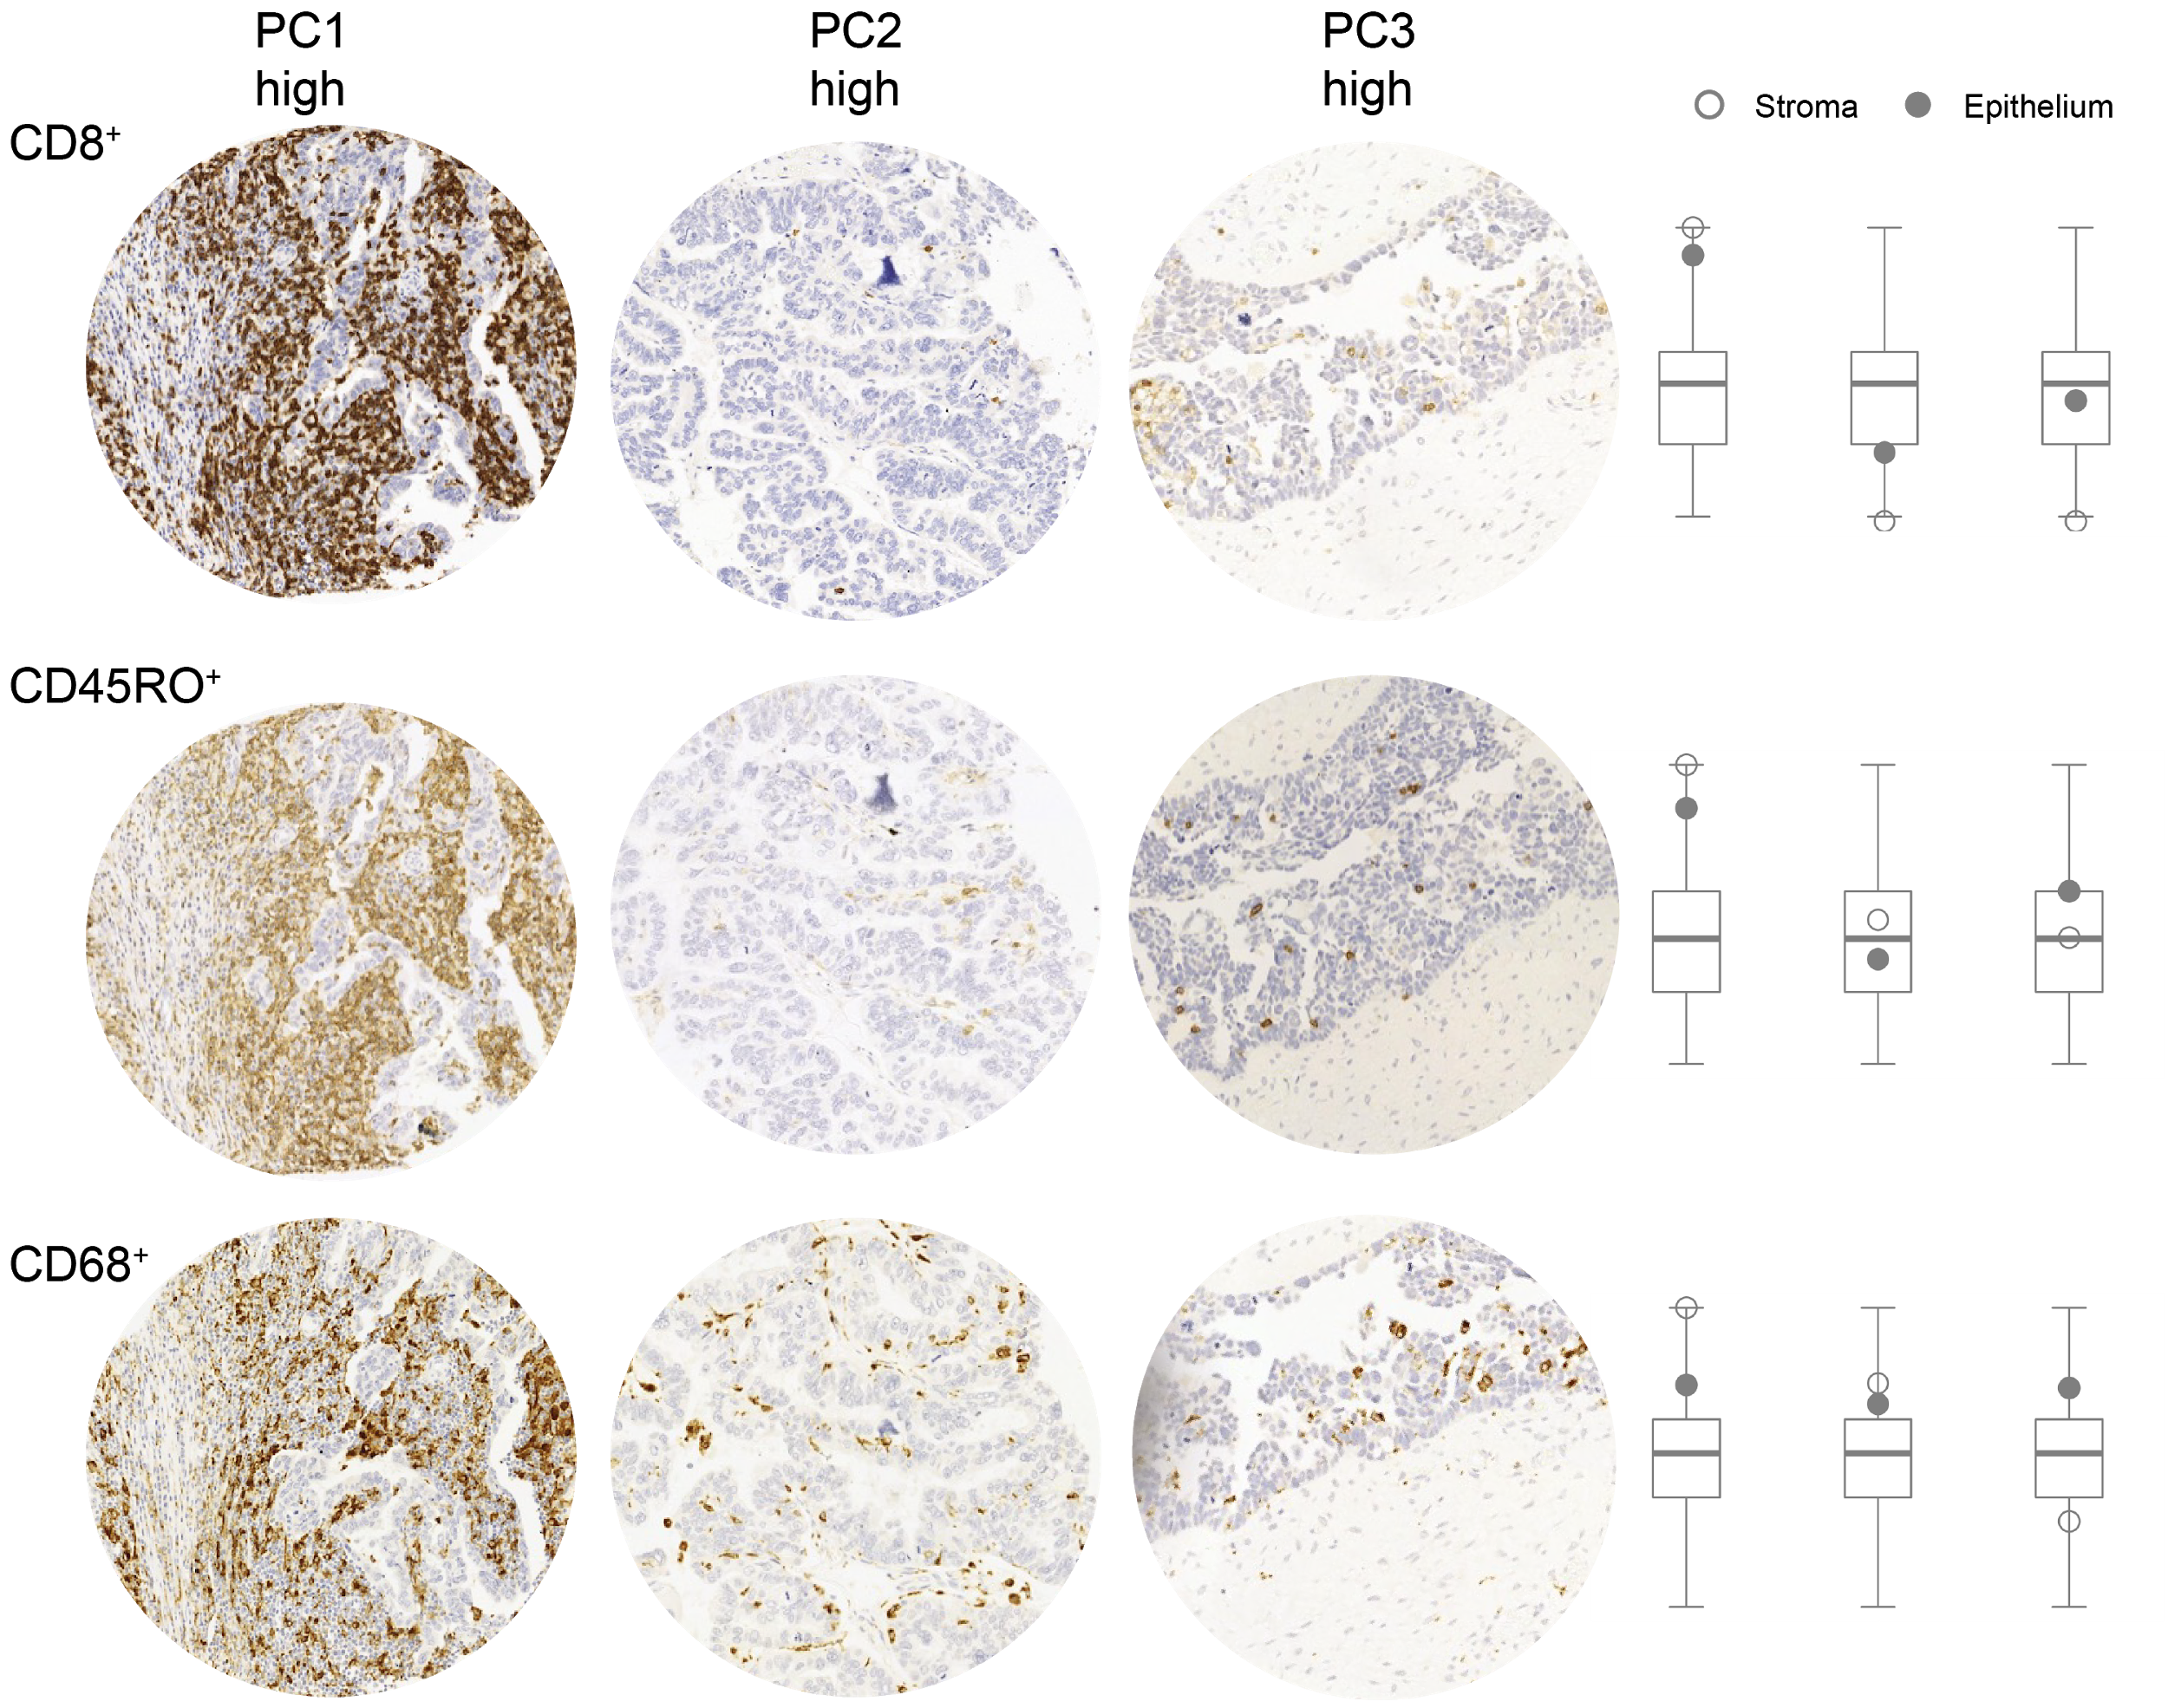
\includegraphics[width=\textwidth]{Chapter2/Figs/Raster/PC_montfort.png}
    \caption[Examples of tissue sections with largest values of principal components.]{Images of the sections of patients with the highest values of principal components 1, 2 and 3. The values of the immune infiltrates of these images are shown on the boxplots of the distribution across all samples.}
    \label{fig:PC_examples}
\end{figure}
\end{landscape}

\begin{figure}
    \centering
    \includegraphics{Chapter2/Figs/Raster/Montfort-2018_Fig7A-PC1.png}
    \caption[Kaplan Meier Curves for Principal Component 1]{Kaplan Meier illustrative survival curve. Principal component 1 are split at the median. The survival of high and low values of Principal component 1 are plotted against time. }
    \label{fig:km_PC}
\end{figure}

\begin{table}[]
    \centering
    \begin{tabular}{lllll} \hline
         	&	\multicolumn{2}{l}{Univariable}			&	\multicolumn{2}{l}{Multivariable}			\\
 	&	HR	&	p-value	&	HR	&	p-value	\\ \hline
PC1	&	0.89	&	0.024	&	0.88	&	0.016	\\
PC2	&	0.94	&	0.61	&	0.92	&	0.52	\\
PC3	&	1.2	&	0.2	&	1.23	&	0.18	\\
PC4	&	1.14	&	0.43	&	1.07	&	0.69	\\
PC5	&	0.82	&	0.31	&	0.74	&	0.11	\\
PC6	&	1.25	&	0.23	&	1.22	&	0.33	\\ \hline

    \end{tabular}
    \caption[Cox proportional hazard regression for principal components]{Cox proportional hazard regression for principal components as predictors. Multivariable analysis includes stage.}
    \label{tab:pc_surv}
\end{table}

\subsection{Comparing Survival Models}
 The Akaike Information Criterion (AIC) was used to compare the performance of these survival models and includes a penalty on the number of terms to reduce over-fitting (Supplementary Fig. 8). The model combining stage, PC1 and PC5 had the best performance for predicting overall survival. The improvement with the addition of PC5 shows that the addition of this principal component has a suppressor effect in the model, increasing the significance of other variables when included. This demonstrates that survival is predominantly determined by the coordinated immune response and further variation in survival from this trend can be encoded by the quantity of epithelial CD45RO$^+$ infiltrate. Interestingly, the models that contained stage and either stromal CD45RO$^+$ or CD68$^+$ infiltrate contained a similar amount of information about patient survival as the one that contained stage and principal components 1 and 5. In our cohort, the density of CD68$^+$ and CD45RO$^+$ stromal infiltrates are therefore the best single infiltrates for survival modelling. 
 
 \begin{figure}
     \centering
     \includegraphics[width=\textwidth]{AIC}
     \caption{AIC for most significant models (AIC > 2)}
     \label{fig:AIC}
 \end{figure}


\subsection{Are genetic defects associated with HGSOC driving individual infiltrates or the coordinated immune response in tumours?}

\subsubsection*{Infiltrate density is not significantly associated with \textit{BRCA} status}
To investigate the interactions between the TME and the genome, can ask whether a germline mutation in either of the \textit{BRCA1/2} genes results in changes in the TME and specifically the immune infiltrate. I investigated whether tumour, stroma or full core measures of CD8$^+$, CD45RO$^+$or CD68$^+$densities were related to \textit{BRCA1/2} mutations using the Kruskal-Wallis rank sum test. I compared the infiltrate density distributions between patients with no mutation, a mutation in \textit{BRCA1} and a mutation in \textit{BRCA2}. I found that the distributions of CD8$^+$, CD45RO$^+$and CD68$^+$infiltrates and the principal components were not significantly associated with \textit{BRCA} mutation status (Figure \ref{fig:genomic}). This was unexpected as previous results have found increases in CD8$^+$infiltrate with a \textit{BRCA1} mutation\cite{Clarke2009}.

\begin{figure}
    \centering
    \includegraphics[width=\textwidth]{Chapter2/Figs/Raster/genomic.png}
    \caption{Boxplots of Infiltrate distribution against genomic phenotype.}
    \label{fig:genomic}
\end{figure}

\subsubsection{Infiltrate density is not significantly associated with type of \textit{TP53} mutation.}
Mutant P53 proteins have been linked to multiple micro-environmental changes\cite{Cordani2016}. I investigated whether the type of TP53 mutation produced measurable changes in the TME. Tumour, stroma or full core measures of CD8$^+$, CD45RO$^+$or CD68$^+$densities were compared between gain or loss of function mutations in \textit{TP53}. I used the Kruskal-Wallis rank sum test and found that the distribution of immune infiltrate was not significantly associated with type of \textit{TP53} mutation.

\subsubsection{Infiltrate density is not significantly associated with change in PTEN expression.}
Changes in PTEN expression are cell-intrinsic and levels of PTEN expression are prognostic in HGSOC\cite{RN17, RN15}. Tumour, stroma or full core measures of CD8$^+$, CD45RO$^+$ or CD68$^+$ densities were compared between patients with high or low PTEN expression as measured by both IHC and IF. Using the Kruskal-Wallis rank sum test I found that change in PTEN expression was not significantly associated with any change in the density of immune infiltrate. This particular cell-intrinsic change is not associated with a change in immune infiltration in our cohort.

The presence of germline \texit{BRCA2} mutations was significantly associated with lower CD8$^+$ cell density than patients with a \texit{BRCA1} after multiple testing correction (Figure \ref{fig:genomic}). There was no significant association between the quantity of CD45RO$^+$ or CD68$^+$ infiltrate and the mutational status of either \texit{BRCA1} or \texit{BRCA2} genes (Figure \ref{fig:genomic}) . No significant association was detected between TP53 GOF and LOF mutations or PTEN expression and the densities of CD8$^+$, CD45RO$^+$ and CD68$^+$ cells in epithelium or stroma (Table \ref{tab:}). Similarly, changes in the principal components were not significantly associated with PTEN expression, TP53 GOF or LOF mutation or germline \textit{BRCA1}/\texit{BRCA2} mutation status (Table \ref{tab:genomic}). 




\begin{table}[]
    \centering
    \begin{tabular}{lllll} \hline
     	&		&	\textit{BRCA1/ BRCA2}	&	p53 GOF/LOF	&	PTEN	\\ \hline
CD8+	&	Epithelium	&	0.04	&	0.54	&	0.67	\\
	&	Stroma	&	0.17	&	0.29	&	0.07	\\
	&	Average	&	0.17	&	0.53	&	0.84	\\
CD45RO+	&	Epithelium	&	0.2	&	0.42	&	0.92	\\
	&	Stroma	&	0.46	&	0.84	&	0.82	\\
	&	Average	&	0.1	&	0.36	&	0.87	\\
CD68+	&	Epithelium	&	0.43	&	0.72	&	0.79	\\
	&	Stroma	&	0.78	&	0.85	&	0.65	\\
	&	Average	&	0.68	&	0.66	&	0.41	\\
Principal Component	&	1	&	0.81	&	0.8	&	0.55	\\
	&	2	&	0.1	&	0.26	&	0.17	\\
	&	3	&	0.27	&	0.58	&	0.51	\\
	&	4	&	0.58	&	0.99	&	0.17	\\
	&	5	&	0.76	&	0.88	&	0.79	\\
	&	6	&	0.97	&	0.44	&	0.18	\\
    \hline
    \end{tabular}
    \caption[Significance of Kruskal Wallis tests of infiltrate against genomic subtype]{P-values associated with Kruskal Wallis test for detecting differences in mean ranks of immune infiltrate in patients grouped by mutation in BRCA1, BRCA2 or not-detected, p53 gof or lof and PTEN high or low in HGSOC.}
    \label{tab:genomic}
\end{table}

\subsection{Other ovarian cancer subtypes}

The automated and reproducible nature of this workflow means similar analyses are easily transposed across to the same immune populations assessed in the other subtypes of Ovarian cancer. Due to the smaller numbers of patients with these subtypes, survival analysis was limited to the X population. Figure \ref{fig:morph_area} shows the areas of epithelium and stroma across all OC subtypes.

\begin{figure}
    \centering
    \includegraphics[width=0.8\textwidth]{Chapter2/Figs/Raster/Morphology_area.png}
    \caption{Area of tumour and stroma across morphological subtypes. (Notches on box plots extend 1.58 ✕ IQR / sqrt(n) and approximate the 95\% confidence interval for the median. Box plot whiskers extend to 1.5 ✕ IQR.) }
    \label{fig:morph_area}
\end{figure}

Figure \ref{fig:morph_immune} shows the distribution of CD45RO$^+$ cells in the stroma and epithelium across the different OC subtypes.

\begin{figure}
    \centering
    \includegraphics{Chapter2/Figs/Raster/CD45RO_morphology.png}
    \caption{Distribution of infiltrate in Stroma and Epithelium for different morphological subtypes of ovarian cancer. (Notches on box plots extend 1.58 ✕ IQR / sqrt(n) and approximate the 95\% confidence interval for the median. Box plot whiskers extend to 1.5 ✕ IQR.) }
    \label{fig:morph_immune}
\end{figure}

\clearpage

\section{Discussion}

The reproducible analysis of quantitative immune data allowed for a rigorous examination of the distributions of immune infiltrates within the SEARCH population and of the potential impacts of localisation of CD8+, CD68+ and CD45RO+ in HGSOC tumours. 

I observed in addition that stromal and epithelial populations and all infiltrates were somewhat positively correlated. This means that samples with low density of stromal immune populations generally had low density of epithelial infiltrate and vice versa. It also meant that patients with high quantities of one infiltrate type often had high infiltration of the others. It is worth noting that the  CD8$^+$ and  CD45RO$^+$ subpopulations are not biologically mutually exclusive and as such I expect some correlation between quantities but in this dataset there was no opportunity to examine the specific spatial locations of the immune cells. 

 One of the key and novel findings of this work was that the global measure of CD8$^+$ infiltrate was a stronger and more significant predictor of survival over CD8$^+$ infiltrate alone. The implication of the average infiltration being a stronger predictor of survival is that averaging over the intra-tumour stroma allows for a better measure of long term infiltration dynamics and measures the presence of a reservoir of immune cells, poised to infiltrate the epithelium.  I also demonstrated here that the quantity of epithelial and stromal CD45RO$^+$ is a positive prognostic feature, a result which also confirms the positive incremental benefit of a long term and mature immune response. 


As discussed in the introduction, many pieces of research have illustrated that macrophage function is micro-environment dependent\cite{ZhangMacrophage2014, li2018intratumoral}, demonstrating that exact localisation effects macrophage function. My work is in agreement with the observation by Li et al. that stromal regions are most prognostic in which to evaluate macrophages. I find however, in contrast to their work in lung cancer, that stromal CD68$^+$ macrophages are a positive prognostic feature. this is further evidence for distinct phenotypes of macrophages between tissue regions. The impact of specific immune cells can vary between cancer types and so further elucidation of the nature of macrophages in HGSOC and their interaction with the TME is required.


I investigated the concept of immune exclusion across this quantitative data set and found that the extent of exclusion was normally distributed. Such a distribution implies that there is not a one-directional process favouring exclusion. I found that the ratio of epithelial:stromal macrophages was prognostic, with increased epithelial macrophage:stroma macrophage ratio having a negative impact upon survival. I would have expected that the quantity of t-cell infiltration from the stromal to intra-epithelial regions would have effected tumour progression and hence survival but given this data I would assert that as the ratio is not prognostic and that the average of the t-cell subsets over the core is prognostic, that there is no explicit long term exclusion of cells, the infiltration at the tumour interface is dynamic and random and that the overall quantity in the larger region is more important than exclusion, which if it is an active process, was not observed to any extreme in this cohort.

Using quantitative data also allowed me see that there was no clear threshold for immune exclusion, but that a 10 fold difference in immune infiltration could be examined for comparisons. I observed that CD8$^+$,  CD45RO$^+$ and  CD68$^+$  infiltrates predominantly exist on a continuum without clear justification for cutpoints.

These observations all suggest that despite the focus of many studies being the intra-epithelial immune infiltration, perhaps due to a focus on direct contact and cytotoxic interaction between immune and tumour cells, that stromal infiltrate should also be evaluated, even in the case of CD8+ t-cell infiltration, to evaluate a larger area and obtain more accurate counts more easily. For macrophages it appears that stromal infiltration plays its own role in the immune response. In the case of the T-cell subsets evaluated here, the stromal region appears to provide more information about the epithelial infiltration as we can infer some element of the longer term immune infiltration dynamics.

In this chapter I also developed the concept of the immunospace. The immunospace views the quantity of each immune infiltration as part of a multidimensional immune landscape for a patient. This approach allowed me to analyse patterns across different immune populations and to derive the principal components as measures of variation. I observed that the correlation between infiltrates amounts to general coordinated immune response which is a positive prognostic. It also allowed me to examine the independence of other phenomenon such as the immune exclusion from the epithelium which was obtained as an axis of variation in an unbiased manner. Such high dimensional methods will be of importance when assessing higher dimensional data sets such as IMC. 


Having reduced the survival analysis to cores that contained epithelium and stroma in order to compare survival impact, the limitation of this analysis is that it assesses the impact of these immune cells within a stromally infiltrated environment. In order to address this I compared the survival impact of CD8 and CD45RO+ in the subset of cores with >99\% epithelium. CD45RO+ was no longer associated with survival which may imply a variation in the functionality of these cells which depends upon their spatial location (within tumour nest).

This work also finds no link between immune infiltration and germline \textit{BRCA} mutations, this is in part due to effects of cohort size. With approximately 20 patients with mutations, I am underpowered to ask multiple questions about the differences in immune infiltration between non-\textit{BRCA} and \textit{BRCA}-mutated patients.

The exact spatial nature of immune infiltration when taking into account tumour structure is unknown. There may also be a link between stromal immune infiltration and collagen deposition. Comparisons of immune infiltration to that which would be expected from diffusion into the epithelium alone has not been examined and is a key questions in the rest of this thesis.

